%!TEX root = ../document.tex
\chapter{Buffer Overflow}
Ein Buffer Overflow ist ein Angriff, bei dem einem Puffer zu viele Werte übergeben werden. Dadurch ist es möglich die Werte anderer Variablen oder Adressen zu überschreiben. \\
Im folgenden Kapitel wird die Portierung und Weiterentwicklung der Buffer Overflow Beispiele aus dem Wintersemester 16/17 auf die Broken Web Application des diesjährigen Semesters beschrieben.

Hierbei wurden die Beispielangriffe um Erklärungen und Anleitungen erweitert, sowie eine Übersichtsseite eingefügt. Auch die angreifbaren Files wurden leicht verändert, so dass auch ohne einen Debugger verständlich ist, wie diese Angriffsart funktioniert.
\section{Übersichtsseite}
Auf der Übersichtsseite wird die generelle Funktion eines Buffer Overflow Angriffs erklärt. Des Weiteren wird ein sehr berühmter Angriff, der Heartbleed - Angriff, in einem Comic mit Erklärung erläutert. Die Übersichtsseite ist in folgender Grafik dargestellt.

\begin{figure}[H]
	\centering
	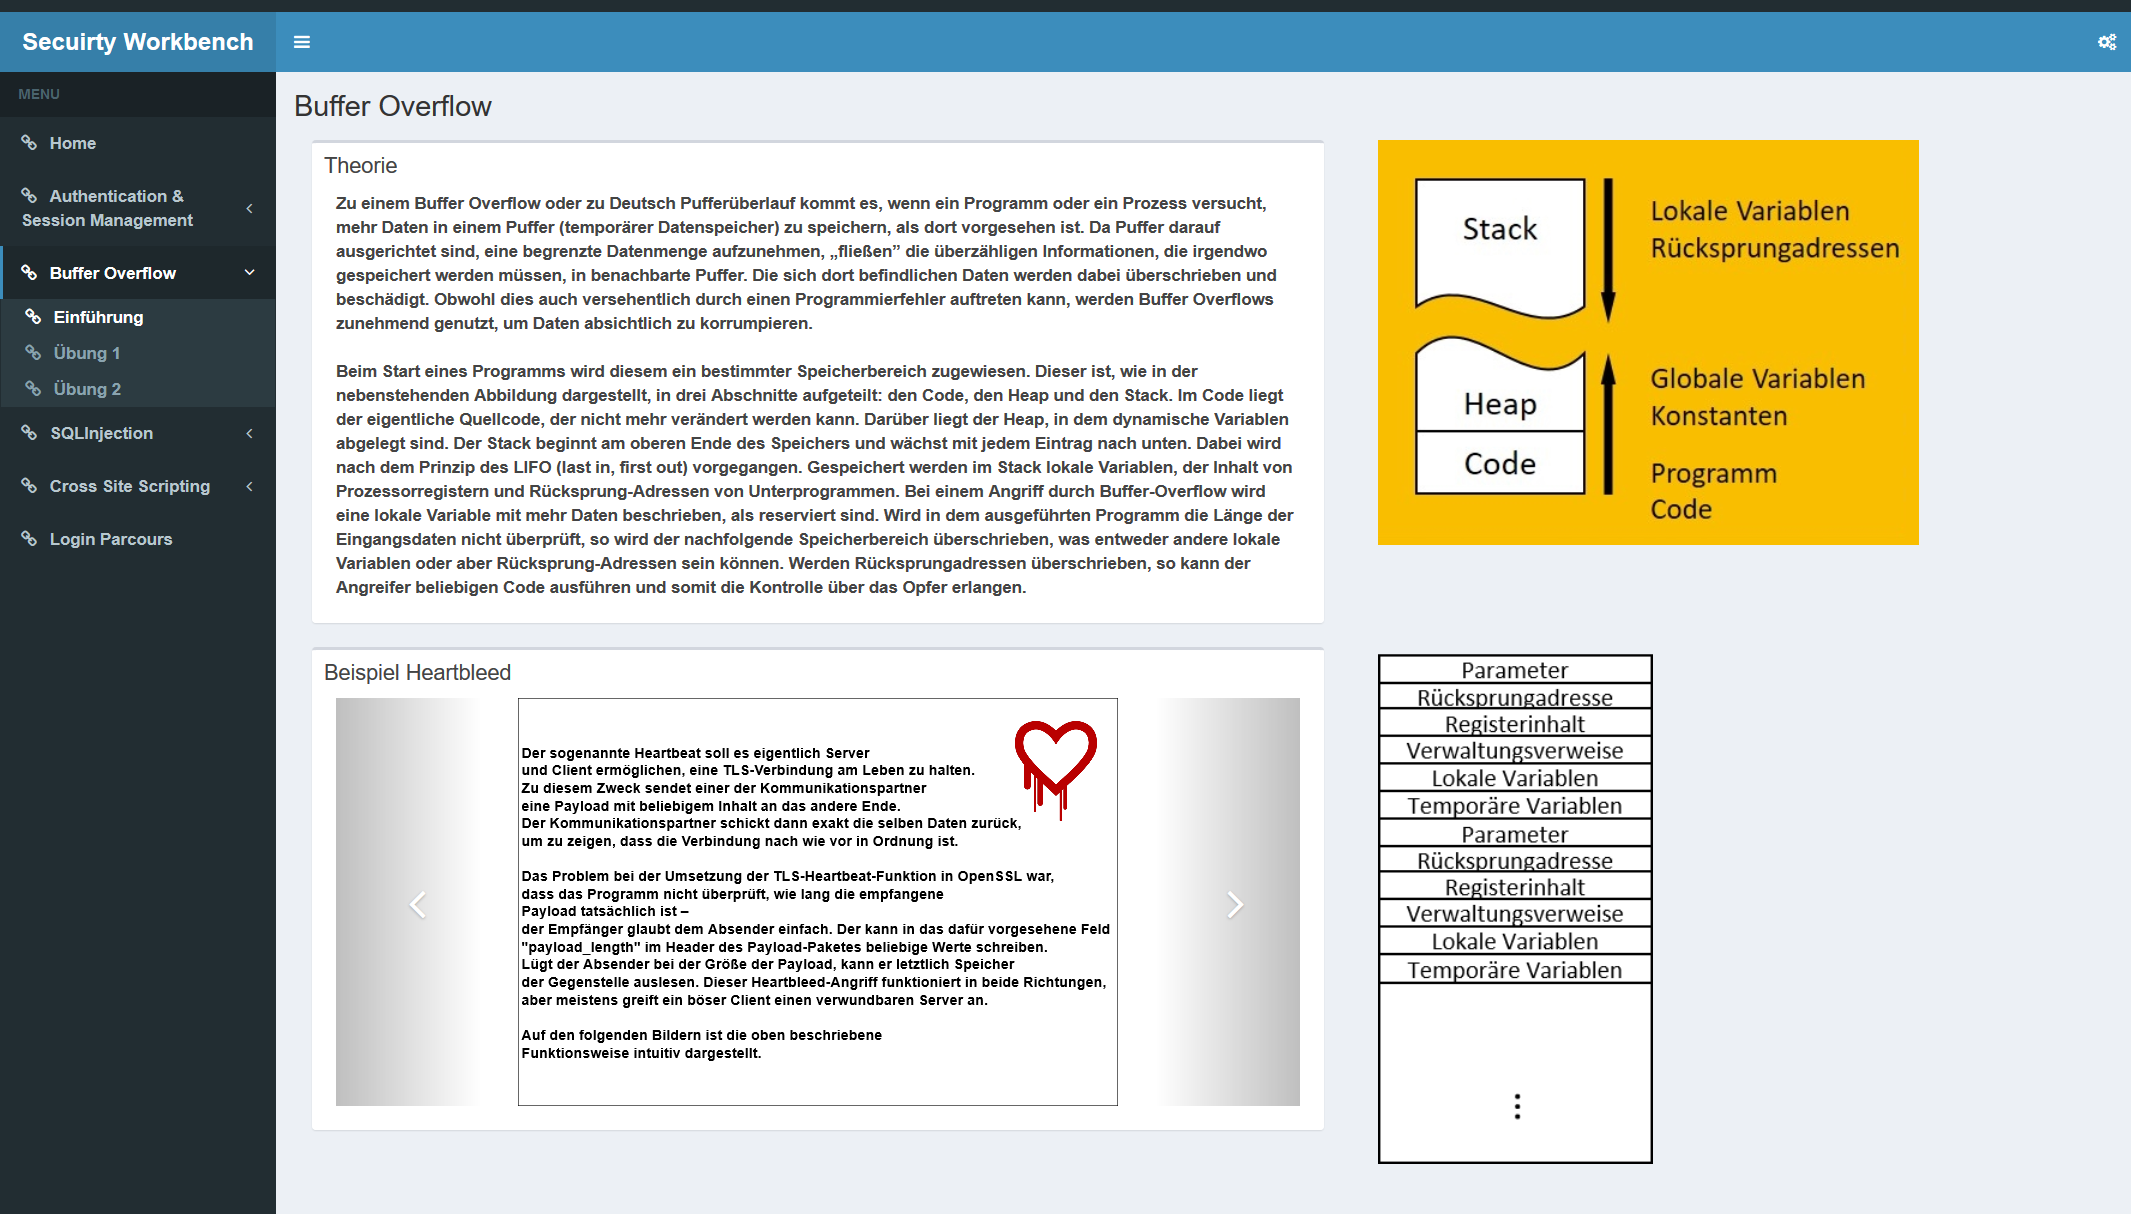
\includegraphics[width=\textwidth]{images/Bufferoverflow/Uebersichtsseite.PNG}
	\caption{Die Übersichtsseite der Buffer Overflow Übungen}
	\label{fig:BO_Overview}
\end{figure}

\section{Übung 1}
\subsection{C-File}
Die erste Übung ist ein sehr einfacher Buffer Overflow. Ein Eingabeparameter wird mit einem zufällig generierten Passwort verglichen und sollten sie identisch sein, wird ein Authentifizierungsflag gesetzt und man hat sich \glqq{}authentifiziert\grqq{}. Dies wird durch eine Erfolgsmeldung und das Ausgeben der Eingabeparameter und Variablen simuliert. Ziel der Übung ist es sich ohne Kenntnis des Passworts zu authentifizieren.
Der Code wird in folgendem Listing dargestellt.

\lstset{language=C, caption={Erstes Buffer Overflow Beispiel}, label=lst:BO_FE}
\begin{lstlisting}
int main(int argc, char *argv[80])
{
    //flag for authentication check
    int authflag = 0;
    //buffer for solution word
    char solution[21];
    //buffer for user input
    char buffer[8];

    //write user input to buffer
    strcpy(buffer, argv[1]);

    char randstr[8];
    srand ( time(NULL) );

    //create random Password
    sprintf(randstr, "%d", rand() );

    //check if input = Password
    if(strcmp(randstr,buffer)== 0)
    {
        printf("Really...?\n");
        //yeah we got the right pw so we are now authenticated
        authflag = 1;
    }

    //check for Authentication
    if(authflag != 0)
    {
        printf("Das Passwort ist: %s\n", randstr);

        printf("Der Eingabepuffer ist: %s\n", buffer);

        printf("Das Authflag hat den Wert: %d\n", authflag);

        printf("Das Lösungswort ist : %s\n", solution);
    }
    else
    {
        printf("Fehler: Login fehlgeschlagen!");
    }
}
\end{lstlisting}
Im Vergleich zu letztem Semester wurde das C-File ein wenig verändert, die Änderungen sind im Folgenden aufgelistet.
\begin{itemize}
	\item \textbf{Seed der Funktion rand()} In der Programmiersprache C ist es nur sehr schwer möglich Zufallszahlen zu generieren. Die gebräuchlichste Methode ist dabei die Funktion rand(), die allerdings auch keine echten Zufallszahlen erzeugt, für dieses Beispiel jedoch ausreichend ist. Wichtig bei der Benutzung dieser Funktion ist indes, dass sie einem sogenannten Seed, der vor Aufruf der Funktion rand() gesetzt werden muss, einen \glqq{}zufälligen\grqq{} Wert zuweist. Das bedeutet, dass die Funktion für den gleichen Seed immer den gleichen Rückgabewert lieft. \\
	Hier hatte das Team des letzten Semesters vergessen den Seed bei jedem Aufruf des Programms zu verändern. In der jetzigen Version wurde deshalb in der Zeile 14 des Programms ein Seed mit der aktuellen Systemzeit gesetzt.
	\item \textbf{Ersetzen des alten Lösungsworts} War der Angriff erfolgreich, so wurde in der alten Version ein Lösungswort ausgegeben. Der Speicherplatz dafür war allerdings mithilfe der Funktion malloc() dynamisch alloziert und damit liegt das Lösungswort auf dem Heap und nicht auf dem Stack, der in diesem Beispiel angegriffen wird. DAs Lösungswort war also nicht überschreibbar und hatte in seinem initialzustand leider keine Bedeutung. \\
	Dieses Lösungswort wurde durch eine Aussagekräftige Ausgabe ersetzt (siehe Zeilen 30ff).
	\item \textbf{Einfügen einer Fehlermedlung} Im alten Programm gab es keine Rückmeldung, sollte der Angriff gescheitert sein. Wird das Programm lokal in einem Debugger ausgeführt, ist das auch kein Problem, da hier eindeutig ersichtlich ist, dass das Programm läuft. Für die Ausführung mithilfe einer Client / Server Architektur, wo in erster Instanz kein Debugger zur Verfügung stand, ist eine Fehlermeldung als Bestätigung des Fehlschlags sehr hilfreich. Diese wurde in der Zeile 40 eingefügt.
\end{itemize}

Um den Angriff erfolgreich durchzuführen, ist es lediglich nötig als Eingabeparameter einen mindestens 30 Zeichen langen String zu übergeben. Dies ist natürlich ein sehr einfaches Beispiel, allerdings spiegelt es sehr gut wider, welche gravierenden Auswirkungen ein einfacher Programmierfehler haben kann.

\subsection{Website}
Auf der Übungsseite befindet sich eine kurze Erklärung des Beispiels, sowie der Code des Programms, der mithilfe von prism direkt aus dem C-File ausgelesen wird. Über die weiter unten befindliche Eingabemaske kann der Angriff ausgeführt werden. Die Ausgabe des Programms wird in der nebenstehenden Box angezeigt. Das Programm wird mit php auf dem Server ausgeführt, der String des Eingabefelds wird per Formular zur Verfügung gestellt.

Sollte das Beispiel für die Studierenden nicht lösbar sein, ist eine dreistufige Tippstruktur vorgesehen, in der den Studierenden je nach Level abstrakte Hinweise gegeben werden, bzw. die Lösung verraten wird.

\subsection{PHP-Shell}
Die integrierte PHP-Shell, soll dem Anwender eine Möglichkeit bieten, den Programmablauf und die Speicherstruktur mit verfolgen zu können. Die PHP-Shell lässt sich wie ein Linux Terminal bedienen. Dazu kann im Eingabefeld das Bash-Kommando eingegeben und mit einem Klick auf den Button \glqq execute command\grqq\, auf dem Server ausgeführt werden. Hierbei werden die Daten mittels POST an den Server geschickt. Der Server startet dabei ein Terminal mit dem entsprechenden Kommando und schließt diesen Prozess nach der Abarbeitung der Befehle. Dabei ist zu beachten, dass das Terminal unter Root-Rechten ausgeführt wird.\medskip

Für dieses Beispiel ist der Gnu Debugger (GDB) hilfreich, um die Speicheradressen der zu überschreibenden Variablen heraus zu finden. Damit kann die Größe der Variablen und somit auch die Länge der Eingabe ermittelt werden. Dies kann z. B. durch folgendes Kommando angezeigt werden:

\bashCommand{gdb -q -batch -ex \glqq break 15\grqq\, -ex \glqq run\grqq\, -ex \glqq p \&authflag\grqq\, -ex \glqq p \&buffer\grqq}\\ \bashCommand{./App\_Data/FirstExample}\medskip

Die oben stehende Anweisung veranlasst, dass in Zeile 15 des Codes ein Breakpoint gesetzt wird. Dabei werden keine Aufrufparameter übergeben, es wird lediglich die Adressen der Variablen authflag und buffer ausgegeben. Hier gilt es zu beachten, dass die Shell nach jedem Ausführen von Kommandos wieder geschlossen wird. Daher muss der GDB im Batch-Modus bedient werden. 

\section{Übung 2}
\subsection{C-File}
Die zweite Übung ist im Vergleich zur ersten ein wenig schwieriger gestaltet. Die Länge des Eingabepuffers wird zwar immer noch nicht überprüft, aber als erste Maßnahme gegen einen Angriff wurde eine Magic Number als Prüfinstanz eingefügt. Diese wurde so platziert, dass sie bei einem Buffer Overflow vor dem Authentifizierungsflag liegt. Damit muss ein Angriff auch diese Magic Number überschreiben. Die restliche Funktion des Programms ist identisch zum ersten Beispiel. \\
Der Code des zweiten Beispiels wird in folgendem Listing dargestellt.

\lstset{language=C, caption={Zweites Buffer Overflow Beispiel}, label=lst:BO_SE}
\begin{lstlisting}
int main(int argc, char *argv[])
{
	//flag for authentification check
	int authflag = 1111;
	int checkForHack = -559038737;

	//buffer for userinput
	char buffer[20];

	//write userinput to buffer
	strcpy(buffer, argv[1]);

	char randstr[20];
	srand ( time(NULL) );
	
	//create random Password
	sprintf(randstr, "%d", rand());

	//check if input = Password
	if(strcmp(randstr,buffer)== 0)
	{
		printf("really\n");
		//yeah we got the right pw so we are now authenticated
		authflag = 1;
	}

	if(checkForHack == -559038737)
	{
		//check for Authentication
		if(authflag != 1111)
		{
			printf("Das Passwort ist: %s\n", randstr);
			
			printf("CheckForHack hat den Wert: %d\n", checkForHack);

			printf("Der Eingabepuffer ist: %s\n", buffer);

			printf("Das Authflag hat den Wert: %d\n", authflag);
		}
	}
	else
	{
		printf("CheckForHack hat den Wert: %d\n", checkForHack);
		printf("Hacker detected; Exit program!\n");
	}

}
\end{lstlisting}
Im Vergleich zum letzten Semester wurden auch am zweiten Beispiel einige Änderungen durchgeführt. Die meisten sind analog zum ersten Beispiel und deshalb in diesem Kapitel nur erwähnt und nicht weiter beschrieben.
\begin{itemize}
	\item \textbf{Seed der Funktion rand()}
	\item \textbf{Ersetzen des alten Lösungsworts}
	\item \textbf{Anpassen der Fehlermeldung} In dem zweiten Beispiel war im Gegensatz zum ersten bereits eine Fehlermeldung für den Fall, dass die Überprüfung der Magic Number fehlschlägt, vorgesehen. Hier wurde dem Studierenden eine kleine Hilfestellung gegeben, indem der Wert der Magic Number Variable auch im Fehlerfall ausgegeben wird.
\end{itemize}
Mit der Einführung der Prüfinstanz werden die Studierenden vor eine neue Herausforderung gestellt, da es jetzt nicht mehr genügt, den Eingabepuffer zum Überlauf zu bringen. Jetzt muss zusätzlich an der richtigen Stelle der Wert der Variable \glqq{}checkForHack\grqq{} stehen, so dass die Variable mit demselben Wert überschrieben wird.\\
In diesem Fall hat die Variable den Wert -559038737 oder 0xDEADBEEF. Diese Werte liegen paarweise in umgekehrter Reihenfolge auf dem Stack (0xEFBEADDE) und müssen dann mit den Unicode Zeichen, die diesen Werten entsprechen überschrieben werden (ï¾­Þ). Hierbei ist zu beachten dass das Unicode Zeichen 0xAD nicht sichtbar dargestellt wird.

\subsection{Website}
Auf der Weboberfläche der zweiten Übung befindet sich ebenfalls eine kurze erklärende Einleitung zur Aufgabe, der Code des Programms, sowie die Tippstruktur und die Ein-, bzw. Ausgabefelder. Auch hier wird dem Programm mithilfe eines Formulars ein Eingabestring übergeben und das Programm wird mittels php auf dem Server ausgeführt.